\documentclass[landscape,a4paper]{article}
\usepackage{commath}
\usepackage{esvect}
\usepackage{xcolor}
\usepackage{graphicx}
\usepackage{gensymb}
\usepackage{mathtools}
\usepackage{amsfonts}
\usepackage{wasysym}
\usepackage{MnSymbol}
\usepackage{IEEEtrantools}
\usepackage{calc}
\usepackage{physics}
\usepackage{siunitx}
\sisetup{product-symbol = \ensuremath{\cdot}}
\sisetup{inter-unit-product = \ensuremath{{}\cdot{}}}
\usepackage{fixdif}
\usepackage{tabularx}
\usepackage{array}
\usepackage{multirow}
\usepackage{booktabs}
\usepackage{xfrac}
\usepackage{indentfirst}
\usepackage{multicol}
\usepackage{parcolumns}
\usepackage[utf8]{inputenc}
\usepackage[T1]{fontenc}
\usepackage[french]{babel}
\usepackage[thinc]{esdiff}
\usepackage{xfrac}
\usepackage[margin=0.5cm]{geometry}
\usepackage[fontsize=7pt]{fontsize}
\usepackage{tikz}
\usetikzlibrary{calc}
\usetikzlibrary{arrows.meta}
\usepackage[tiny]{titlesec}
\titlespacing{\section}{0pt}{*0.5}{*0.3}
\titlespacing{\subsection}{0pt}{*1}{*2}
\titlespacing{\subsubsection}{0pt}{*0.4}{*0.5}

\newcommand{\eqentry}[1]{\(\displaystyle #1\)}
\pagestyle{empty}

\newcommand{\req}[2]{
  \begin{center}
    \scalebox{#1}{
      \begin{tabular}{c}
        \(\displaystyle
        #2
        \)
      \end{tabular}
    }
  \end{center}
}

\newcommand{\dee}[1]{
  \,\,\,\mathrm{d}{#1}
}

\newcommand{\dx}{ \dee x }
\newcommand{\dt}{ \dee t }

\newcommand{\veca}{\vv{a}}
\newcommand{\vecb}{\vv{b}}
\newcommand{\vecc}{\vv{c}}

\newcommand{\F}{\ensuremath{\vv{F}}}

\newcommand{\Qm}{\ensuremath{\vv{P}}}
\newcommand{\qm}{\ensuremath{\vv{p}}}

\newcommand{\pos}{\ensuremath{\vv{r}}}
\newcommand{\vi}{\ensuremath{\vv{v}}}
\newcommand{\vian}{\ensuremath{\vv{\omega}}}
\newcommand{\Vian}{\ensuremath{\vv{\Omega}}}

\newcommand{\ac}{\ensuremath{\vv{a}}}

\newcommand{\eva}{\bigg|}

\newcommand{\ux}{\ensuremath{\vv{u}_x}}
\newcommand{\uy}{\ensuremath{\vv{u}_y}}
\newcommand{\uz}{\ensuremath{\vv{u}_z}}

\newcommand{\ur}{\ensuremath{\vv{u}_{r}}}
\newcommand{\utheta}{\ensuremath{\vv{u}_{\theta}}}
\newcommand{\uphi}{\ensuremath{\vv{u}_{\varphi}}}
\newcommand{\urho}{\ensuremath{\vv{u}_{\rho}}}

\newcommand{\mc}{\ensuremath{\vv{L}}}
\newcommand{\mf}{\ensuremath{\vv{M}}}

\newcommand{\exte}{\text{ext}}
\newcommand{\inte}{\text{int}}

\newcommand{\ti}{\ensuremath{\widetilde{I}}}

\newcommand{\refe}{\mathcal{R}}

\newcommand{\nod}{\vv{n}}

\newcommand{\eqligne}[3]{\(\displaystyle #2\) & \(\displaystyle #1\) & \(\displaystyle#3\) \\}
\newcommand{\trigo}[3]{\(\displaystyle #1\) & \(\displaystyle #2\) & \(\displaystyle#3\) \\}
\newcommand{\trigod}[2]{\(\displaystyle #1\) & \(\displaystyle #2\) \\}

\newcommand{\Sin}[1]{\sin\left(#1\right)}
\newcommand{\Cos}[1]{\cos\left(#1\right)}
\newcommand{\Tan}[1]{\tan\left(#1\right)}
\newcommand{\Sins}[1]{\sin^2\left(#1\right)}
\newcommand{\Coss}[1]{\cos^2\left(#1\right)}
\newcommand{\Tans}[1]{\tan^2\left(#1\right)}
\newcommand{\Cot}[1]{\cot\left(#1\right)}
\newcommand{\Arcsin}[1]{\arcsin\left(#1\right)}
\newcommand{\Arccos}[1]{\arccos\left(#1\right)}
\newcommand{\Arctan}[1]{\arctan\left(#1\right)}

\begin{document}
\begin{multicols}{4}
  \section{Intro mathématique}
  \renewcommand{\arraystretch}{2} % Augmente l'espacement des lignes de 50%
  % \subsection{Logarithmes}
  % \[
  %   y=\log_a(x) \Leftrightarrow a^y = x
  % \]
  % \[
  %   \log_a(xy) = \log_a(x) + \log_a(y)
  % \]
  % \[
  %   \log_a\left(\frac{x}{y}\right) = \log_a(x) - \log_a(y)
  % \]
  % \[
  %   \log_a\left(\frac{1}{x}\right) = -\log_a(x)
  % \]
  % \[
  %   \log_a\left(x^p\right) = p\log_a(x)
  % \]
  % \[
  %   y=\log(x) \Leftrightarrow 10^y = x 
  % \]
  % \[
  %   y=\ln(x) \Leftrightarrow e^y = x 
  % \]
  %
  % Changement de base : 
  % \[
  %   \log_a(x)=\frac{\log_b(x)}{\log_b(a)}=\frac{\log(x)}{\log(a)}=\frac{\ln(x)}{\ln(a)}
  % \]

  \subsection{Trigo}
  \begin{center}
    \begin{tabular}{cc}
      \trigod{\cos^2(\alpha) + \sin^2(\alpha) = 1}{ \tan(\alpha)=\frac{\sin(\alpha)}{\cos(\alpha)}=\frac{1}{\cot(\alpha)}}
      \trigod{ \frac{1}{\cos^2(\alpha)}=1+\tan^2(\alpha)}{ \frac{1}{\sin^2(\alpha)}=1+\cot^2(\alpha)}
    \end{tabular}
    \vspace{0.1cm}\hrule\vspace{0.1cm}
    \scalebox{0.75}{
      \begin{tabular}{ccc}
        % \toprule
        \trigo{\Cos{\alpha+2\pi}=\Cos{\alpha}}{\Sin{\alpha+2\pi}=\Sin{\alpha}}{\Tan{\alpha+\pi}=\Tan{\alpha}}
        % \midrule
        \trigo{\Cos{-\alpha}=\Cos{\alpha}}{\Sin{-\alpha}=-\Sin{\alpha}}{\Tan{-\alpha}=-\Tan{\alpha}}
        \trigo{\Cos{\pi-\alpha}=-\Cos{\alpha}}{\Sin{\pi-\alpha}=\Sin{\alpha}}{\Tan{\pi-\alpha}=-\Tan{\alpha}}
        \trigo{\Cos{\pi+\alpha}=-\Cos{\alpha}}{\Sin{\pi+\alpha}=-\Sin{\alpha}}{\Tan{\pi+\alpha}=\Tan{\alpha}}
        \trigo{\Cos{\frac{\pi}{2}-\alpha}=\Sin{\alpha}}{\Sin{\frac{\pi}{2}-\alpha}=\Cos{\alpha}}{\Tan{\frac{\pi}{2}-\alpha}=\Cot{\alpha}}
        \trigo{\Cos{\frac{\pi}{2}+\alpha}=-\Sin{\alpha}}{\Sin{\frac{\pi}{2}+\alpha}=\Cos{\alpha}}{\Tan{\frac{\pi}{2}+\alpha}=-\Cot{\alpha}}
        % \bottomrule
      \end{tabular}
    }
    \vspace{0.1cm}\hrule\vspace{0.1cm}
    \scalebox{0.6}{
      \begin{tabular}{cc}
        % \toprule
        \trigod{\Cos{\alpha+\beta}=\Cos{\alpha}\Cos{\beta}-\Sin{\alpha}\Sin{\beta}}{\Cos{\alpha-\beta}=\Cos{\alpha}\Cos{\beta}+\Sin{\alpha}\Sin{\beta}}
        \trigod{\Sin{\alpha+\beta}=\Sin{\alpha}\Cos{\beta}+\Cos{\alpha}\Sin{\beta}}{\Sin{\alpha-\beta}=\Sin{\alpha}\Cos{\beta}-\Cos{\alpha}\Sin{\beta}}
        \trigod{\Tan{\alpha+\beta}=\frac{\Tan{\alpha}+\Tan{\beta}}{1-\Tan{\alpha}\Tan{\beta}}}{\Tan{\alpha-\beta}=\frac{\Tan{\alpha}-\Tan{\beta}}{1+\Tan{\alpha}\Tan{\beta}}}
        % \bottomrule
      \end{tabular}
    }
    \vspace{0.1cm}\hrule\vspace{0.1cm}
    \scalebox{0.9}{
      \begin{tabular}{l}
        % \toprule
        \(\displaystyle\Cos{2\alpha}=\Coss{\alpha}-\Sins{\alpha}=1-2\Sins{\alpha}=2\Coss{\alpha}-1\)\\
        \(\displaystyle\Sin{2\alpha}=2\Sin{\alpha}\Cos{\alpha}\)\\
        \(\displaystyle\Tan{2\alpha}=\frac{2\Tan{\alpha}}{1-\Tans{\alpha}}\)\\
        % \bottomrule
      \end{tabular}
    }
    \vspace{0.1cm}\hrule\vspace{0.1cm}
    \scalebox{0.8}{
      \begin{tabular}{cc}
        % \toprule
        \trigod{\Coss{\frac{\alpha}{2}}=\frac{1+\Cos{\alpha}}{2}}{\Sins{\frac{\alpha}{2}}=\frac{1-\Cos{\alpha}}{2}}
        \trigod{\Tans{\frac{\alpha}{2}}=\frac{1-\Cos{\alpha}}{1+\Cos{\alpha}}}{\Tan{\frac{\alpha}{2}}=\frac{1-\Cos{\alpha}}{\Sin{\alpha}}=\frac{\Sin{\alpha}}{1+\Cos{\alpha}}}
        % \bottomrule
      \end{tabular}
    }
    \vspace{0.1cm}\hrule\vspace{0.1cm}
    \scalebox{0.6}{
      \begin{tabular}{cc}
        \trigod{
          \Cos{\alpha}+\Cos{\beta}=2\Cos{\frac{\alpha+\beta}{2}}\Cos{\frac{\alpha-\beta}{2}}
        }{
          \Cos{\alpha}-\Cos{\beta}=-2\Sin{\frac{\alpha+\beta}{2}}\Sin{\frac{\alpha-\beta}{2}}
        }
        \trigod{
          \Sin{\alpha}+\Sin{\beta}=2\Sin{\frac{\alpha+\beta}{2}}\Cos{\frac{\alpha-\beta}{2}}
        }{
          \Sin{\alpha}-\Sin{\beta}=2\Cos{\frac{\alpha+\beta}{2}}\Sin{\frac{\alpha-\beta}{2}}
        }
        \trigod{
          \Tan{\alpha}+\Tan{\beta}= \frac{\Sin{\alpha+\beta}}{\Cos{\alpha}\Cos{\beta}}
        }{
          \Tan{\alpha}-\Tan{\beta}= \frac{\Sin{\alpha-\beta}}{\Cos{\alpha}\Cos{\beta}}
        }
      \end{tabular}
    }
    \vspace{0.1cm}\hrule\vspace{0.1cm}
  \end{center}
  \[
    a\Cos{\alpha} +b\Sin{\alpha} = \sqrt{a^2 + b^2}\Cos{\alpha - \varphi}
  \]
  \[
    \varphi=\Arccos{\frac{a}{\sqrt{a^2 + b^2}}}=\Arcsin{\frac{b}{\sqrt{a^2 + b^2}}}=\Arctan{\frac{b}{a}}
  \]
  % \begin{center} \vspace{0.1cm}\hrule\vspace{0.1cm} \end{center}
  % \begin{align*}
  %   2\Cos{\alpha}\Cos{\beta}&=\Cos{\alpha+\beta} + \Cos{\alpha-\beta}\\
  %   2\Cos{\alpha}\Sin{\beta}&=\Sin{\alpha+\beta} - \Sin{\alpha-\beta}\\
  %   2\Sin{\alpha}\Sin{\beta}&=-\Cos{\alpha+\beta} + \Cos{\alpha-\beta}\\
  % \end{align*}
  % \begin{center} \hrule\vspace{0.1cm} \end{center}
  \[
    \cos(x)=a \Rightarrow
    \begin{cases}
      x = \arccos(a) + k\cdot 2\pi \,\,\,\,\text{ou}\\
      x = - \arcsin(a) + k\cdot 2\pi 
    \end{cases}
  \]

  \[
    \sin(x)=a \Rightarrow
    \begin{cases}
      x = \arcsin(a) + k\cdot 2\pi \,\,\,\,\text{ou}\\
      x = \pi - \arcsin(a) + k\cdot 2\pi 
    \end{cases}
  \]

  \[\tan(x)= a \Rightarrow x = \arctan(a) + k\cdot\pi\]
  % \begin{center} \vspace{0.1cm}\hrule\vspace{0.1cm} \end{center}
  \[
    a^2 = b^2 + c^2 - 2bc\Cos{\alpha}\phantom{text} \frac{a}{\sin(\alpha)}=\frac{b}{\sin(\beta)} 
  \]


  \renewcommand{\arraystretch}{1}

  \subsection{Géométrie}
  \subsubsection{Vecteur}
  \req{1}{
    \ac\cdot\vv{b}=||\ac||\,\,||\vv{b}||\cos\varphi \phantom{textus} ||\ac||=\sqrt{\ac\cdot\ac} 
  }

  Projection de \(\vv{b}\) sur \(\ac\) : 
  \[
    \vv{b}' = \frac{\ac\cdot\vv{b}}{||\ac||^2}\ac \phantom{texttext} 
    ||\ac\times\vv{b}||=||\ac||\,\,||\vv{b}||\sin\varphi
  \]
  \[
    \ac\times\vv{b}=\begin{pmatrix}
      a_2b_3 - a_3b_2 \\ 
      a_3b_1 - a_1b_3 \\ 
      a_1b_2 - a_2b_1
    \end{pmatrix}
    =-(\vecb\times\veca)
  \]
  \[
    \veca\times(\vecb\times\vecc)=(\veca\cdot\vecc)\vecb - (\veca\cdot\vecb)\vecc
  \]

  \subsection{Dérivés et integrales}
  % \subsubsection{Dérivation}
  % \(\displaystyle
  %   f'(x)=\diff{f}{x} \phantom{text} f''(x)=\diff[2]{f}{x} \phantom{text} f^{(n)}(x)=\diff[n]{f}{x}
  % \)
  %
  % \(\displaystyle
  %   (f+g)'(x)=f'(x)+g'(x) \phantom{text} (\lambda\cdot f)'(x)=\lambda f'(x)
  % \)
  %
  % \(\displaystyle
  %   (f\cdot g)'(x)=f'(x)g(x)+f(x)g'(x)
  % \)
  %
  % \(\displaystyle
  %   \left(\frac{f}{g}\right)'(x)=\frac{f'(x)g(x)-f(x)g'(x)}{g^2(x)}
  % \)
  %
  % \(\displaystyle
  %   (g\circ f)'(x)=g'(f(x))f'(x)
  % \)
  % \subsubsection{Intégration}
  % \begin{tabular}{p{1.8cm}l}
  %   \multirow{2}{*}{Linéarité} & \eqentry{ \int(f(x) + g(x))\dx = \int f(x)\dx + \int g(x)\dx } \\ 
  %
  %                              & \eqentry{ \int \lambda f(x)\dx = \lambda\int f(x)\dx } \\
  %
  %   Par parties & \eqentry{ \int f'(x)g(x)\dx = f(x)g(x) - \int f(x)g'(x)\dx} \\
  %
  %   Par substitution & \eqentry{ \int g(f(x))f'(x)\dx = G(x) + c} \\ 
  %
  %   Par changement de variable (\(x=f(t)\)) & \eqentry{ \int g(x)\dx = \int g(f(t))f'(t) \dt } \\
  % \end{tabular}

  % Linéarité : 
  %
  % \(\displaystyle \int(f(x) + g(x))\dx = \int f(x)\dx + \int g(x)\dx \)
  %
  % \(\displaystyle \int \lambda f(x)\dx = \lambda\int f(x)\dx \)

  Par parties : 

  \(\displaystyle \int f'(x)g(x)\dx = f(x)g(x) - \int f(x)g'(x)\dx \)

  Par substitution : 
  \(\displaystyle \int g(f(x))f'(x)\dx = G(x) + c \)

  Par changement de variable (\(x=f(t)\)) : 

  \(\displaystyle \int g(x)\dx = \int g(f(t))f'(t) \dt \)

  \renewcommand{\arraystretch}{2}
  \begin{center}
    \scalebox{0.6}{
      \begin{tabular}{c|c|c}
        \toprule
        \eqligne{f(x)}{f'(x)}{F(x)}
        \midrule
        \eqligne{a}{0}{ax}
        \eqligne{x}{1}{x^2}
        \eqligne{\frac{1}{x}}{-\frac{1}{x^2}}{\ln|x|}
        \eqligne{\sqrt{x}}{\frac{1}{2\sqrt{x}}}{\tfrac{2}{3}x\sqrt{x}}
        \eqligne{\frac{1}{\sqrt{x}}}{-\tfrac{1}{2}\sqrt{x^3}}{2\sqrt{x}}
        \eqligne{x^n}{nx^{n-1}}{\frac{1}{n+1}x^{n+1}}
        \eqligne{\frac{1}{x^{n}}}{\frac{-n}{x^{n-1}}}{\frac{-1}{n-1}\frac{1}{x^{n-1}}}
        \eqligne{\sqrt[n]{x}}{\frac{1}{n}\sqrt[n]{x^{n-1}}}{\frac{n}{n+1}\sqrt[n]{x^{n+1}}}
        % \midrule
        \eqligne{e^{ax}}{ae^{ax}}{\frac{1}{a}e^{ax}}
        \eqligne{b^{ax}}{ab^{ax}\ln(b)}{\frac{b^{ax}}{a\ln(b)}}
        \eqligne{\ln(x)}{\frac{1}{x}}{x(\ln(x) - 1)}
        \eqligne{\log_{a}(bx)}{\frac{1}{x\ln(a)}}{x\log_{a}\left(\frac{bx}{e}\right)}
        % \midrule
        \eqligne{\sin(x)}{\cos(x)}{-\cos(x)}
        \eqligne{\cos(x)}{-\sin(x)}{\sin(x)}
        \eqligne{\tan(x)}{\frac{1}{\cos^2(x)}}{-\ln|\cos(x)|}
        % \eqligne{\sin^2(x)}{2\sin(x)\cos(x)}{\tfrac{1}{2}(x-\sin(x)\cos(x))}
        % \eqligne{\cos^2(x)}{-2\sin(x)\cos(x)}{\tfrac{1}{2}(x+\sin(x)\cos(x))}
        % \eqligne{\tan^2(x)}{2 \frac{\tan(x)}{\cos^2(x)}}{\tan(x) - x}
        % \midrule 
        \eqligne{\arcsin(x)}{\frac{1}{\sqrt{1-x^2}}}{x\arcsin(x) + \sqrt{1-x^2}}
        \eqligne{\arccos(x)}{-\frac{1}{\sqrt{1-x^2}}}{x\arccos(x) - \sqrt{1-x^2}}
        \eqligne{\arctan(x)}{\frac{1}{1+x^2}}{x\arctan(x) - \tfrac{1}{2}\ln(1+x^2)}
        % \midrule
        \eqligne{g(x)g'(x)}{g'(x)^2 +g(x)g''(x)}{\tfrac{1}{2}g(x)^2}
        \eqligne{\frac{g'(x)}{g(x)}}{\frac{g''(x)g(x)-g'(x)^2}{g(x)^2}}{\ln|g(x)|}
        \bottomrule
      \end{tabular}
    }
  \end{center}
  \renewcommand{\arraystretch}{1} % Augmente l'espacement des lignes de 50%
  \subsection{Polynômes Taylor}
  \[
    P_N(x)=\eval{\sum_{n=0}^{N}\frac{1}{n!}\diff[n]{f}{x}}_{x=x_0}(x-x_0)^n
  \]

  \section{Cinématique}

  \[
    \ac(t)=\diff{\vi}{t}=\dot{\vi}=\ddot{\pos}=
    \diff[2]{}{t}\left(x_1\vv{u}_1 + x_2\vv{u}_2 + x_3\vv{u}_3\right)
  \]

  \[
    \ac=\diff{v}{t}\vv{u_t} + v\diff{\vv{u_t}}{t} = \diff{v}{t}\vv{u_t} + \frac{v^2}{R_c}\vv{u_n}
  \]

  \subsection{Coordnonnée cylindrique}
  \begin{center}
    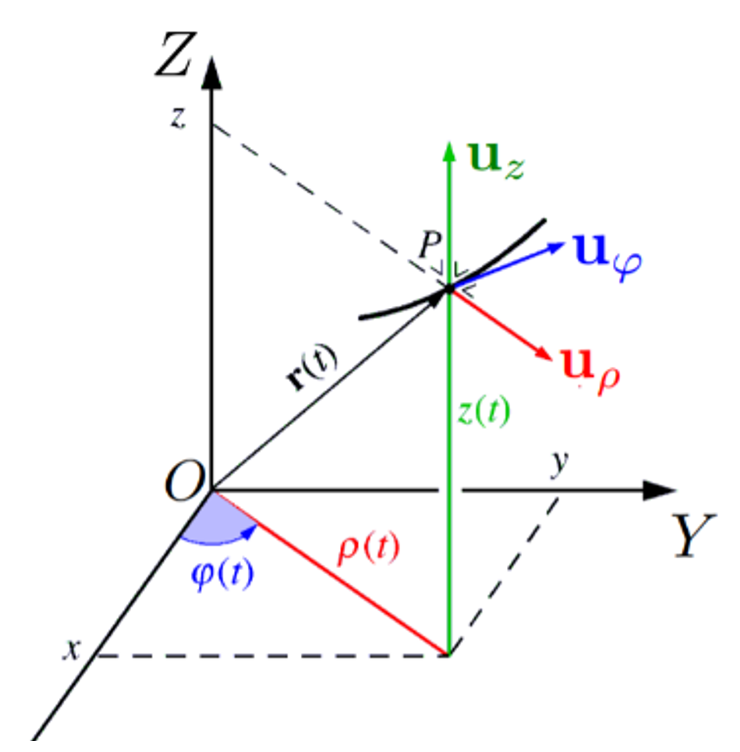
\includegraphics[width=0.1\textwidth]{images/PHYSIQUEI_1.png}
    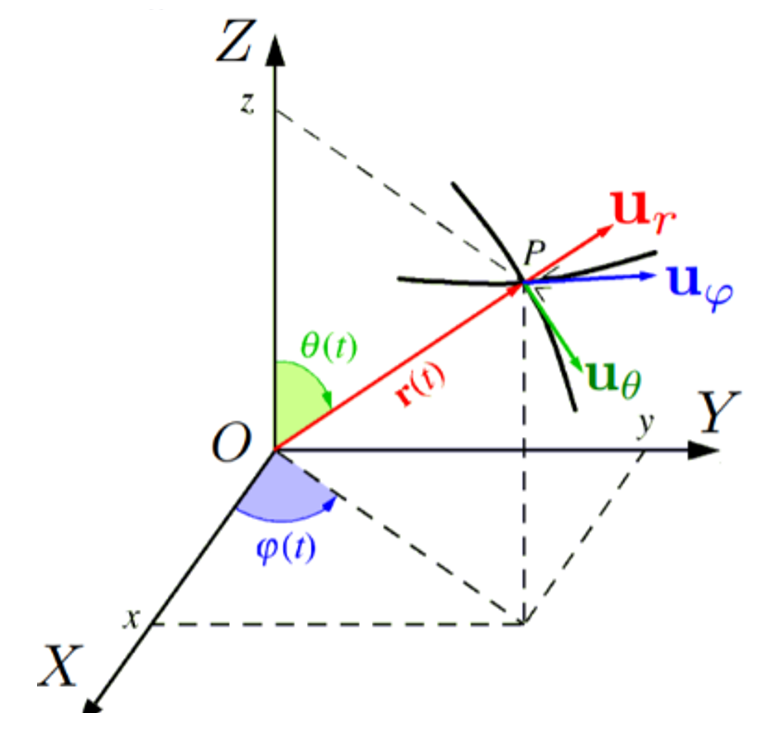
\includegraphics[width=0.1\textwidth]{images/PHYSIQUEI_2.png}
  \end{center}

  \vspace{-0.4cm}
  \begin{IEEEeqnarray*}{rCl}
    \vi
    \begin{cases}
      v_{\rho} = \dot{\rho}\\
      v_{\varphi} = \rho\dot{\varphi}\\
      v_{z} = \dot{z}
    \end{cases}
    &
    \ac
    \begin{cases}
      a_{\rho} = \ddot{\rho} - \rho\dot{\varphi}^2\\
      a_{\varphi} = 2\dot{\rho}\dot{\varphi} + \rho\ddot{\varphi}\\
      a_{z} = \ddot{z}
    \end{cases}
  \end{IEEEeqnarray*}

  \subsection{Coordnonnée sphérique}
  \vspace{-0.3cm}
  \begin{IEEEeqnarray*}{rCl}
    \vi
    \begin{cases}
      v_{r} = \dot{r}\\
      v_{\theta} = r\dot{\theta}\\
      v_{\varphi} = r\dot{\varphi}\sin{\theta}
    \end{cases}
    & \ac
    \begin{cases}
      a_{r} = \ddot{r} - r\dot{\theta}^2 - r\dot{\varphi}^2 \sin^2\theta \\
      a_{\theta} = r\ddot{\theta} + 2\dot{r}\dot{\theta} - r\dot{\varphi}^2 \cos\theta \sin\theta \\
      a_{\varphi} = r\ddot{\varphi} \sin\theta + 2r\dot{\varphi}\dot{\theta} \cos\theta + 2\dot{r}\dot{\varphi} \sin\theta
    \end{cases}
  \end{IEEEeqnarray*}

  \subsection{Changement de base}
  Cartésien-cylindrique : 
  \[
    \begin{array}{ll}
      \vv{u}_{\rho}=\cos\varphi\ux + \sin\varphi\uy &
      \ux = \cos\varphi\vv{u}_{\rho} - \sin\varphi\vv{u}_{\varphi}\\

      \vv{u}_{\varphi}=-\sin\varphi\ux + \cos\varphi\uy &
      \uy = \sin\varphi\vv{u}_{\rho} + \cos\varphi\vv{u}_{\varphi}\\

      \vv{u}_{z}=\vv{u}_{z} & \vv{u}_{z}=\vv{u}_{z}
    \end{array}
  \]

  Cartésien-sphérique : 
  \begin{align*}
    \vv{u}_{r}&=\sin\theta\cos\varphi\vv{u}_{x} + \sin\theta\sin\varphi\vv{u}_{y} + \cos\theta\vv{u}_{z}\\
    \vv{u}_{\theta}&=\cos\theta\cos\varphi\vv{u}_{x} + \cos\theta\sin\varphi\vv{u}_{y} - \sin\theta\vv{u}_{z}\\
    \vv{u}_{\varphi}&=-\sin\varphi\vv{u}_{x} + \cos\varphi\vv{u}_{y}\\\\
    \vv{u}_{x}&=\sin\theta\cos\varphi\vv{u}_{r} + \cos\theta\cos\varphi\vv{u}_{\varphi} - \sin\varphi\vv{u}_{\theta}\\
    \vv{u}_{y}&=\sin\theta\sin\varphi\vv{u}_r + \cos\theta\sin\varphi\vv{u}_{\varphi} + \cos\varphi\vv{u}_{\theta}\\
    \vv{u}_{z}&=\cos\theta\vv{u}_r - \sin\theta\vv{u}_{\varphi}
  \end{align*}

  Cylindrique-sphérique : 
  \[
    \begin{array}{ll}
      \urho = \sin\theta\ur + \cos\theta\utheta &
      \ur =\sin\theta\urho + \cos\theta\uz\\ 

      \uphi = \uphi &
      \utheta = \cos\theta\urho - \sin\theta\uz \\

      \uz = \cos\theta\ur - \sin\theta\utheta &
      \uphi = \uphi
    \end{array}
  \]

  \section{Dynamique}
  \req{1}{
    \sum_i \F_i=m\ac=m\diff[2]{\pos}{t}\phantom{texttex} \F_{1\to 2} = -\F_{2\to 1}
  }

  \subsection{Ressort}
  \req{1}{
    \F_r = -k(x-l_0)\vv{u} \phantom{texttext} U=\tfrac{1}{2}k(x-l_0)^2
  }

  \subsection{Gravitation}
  \req{1}{
    \F_{2\to 1}=-G \frac{m_1m_2}{r_{12}^2} \vv{u}_{2\to 1} \phantom{textte} \F=m\vv{g}
  }

  \subsection{Electromagnétisme}
  \[
    \F_{2\to 1}= \frac{1}{4\pi\epsilon_0}\frac{q_1q_2}{r_{12}^2}\vv{u}_{2\to 1}
  \]

  \[
    \F=q\vv{E} \phantom{texttext} \F=q\vi\times\vv{B}
  \]

  \begin{center}
    \begin{tikzpicture}[scale=0.3,>=Stealth]
      \coordinate (q1) at (0,0);
      \coordinate (q2) at (3,0);

      \draw[dashed] (q1) -- (q2);

      \draw[->] (q2) -- (1.7,0) node[midway, above] {$\vec{u}_{2 \to 1}$};

      \fill[red] (q1) circle(0.2cm);
      \fill[red] (q2) circle(0.2cm);

      \node[left] at (q1) {$q_1$};
      \node[right] at (q2) {$q_2$};
    \end{tikzpicture}\hspace{1cm}
    \begin{tikzpicture}[scale=0.3,>=Stealth]
      \coordinate (q1) at (0,0);
      \coordinate (q2) at (3,0);

      \draw[dashed] (q1) -- (q2);

      \draw[->] (q2) -- (1.7,0) node[midway, above] {$\vec{u}_{2 \to 1}$};

      \fill[red] (q1) circle(0.2cm);
      \fill[red] (q2) circle(0.2cm);

      \node[left] at (q1) {$m_1$};
      \node[right] at (q2) {$m_2$};
    \end{tikzpicture}
  \end{center}
  \subsection{Frottement}

  % \begin{table}
  % \begin{tabular}{p{2cm}|c|l|c}
  %     \toprule
  %     \multirow{2}{*}{Frottement visqueux} & $ \F_{res}=k(l_0 - l)\vv{u}_{r} $ & Régime laminaire & \(f(||\vi_{rel}||)=k\nu||\vi_{rel}||\)\\
  %                                          & $ \F_{rel}=\vi_{obj} - \vi_{fluid} $ & Régime turbulant & c \\
  %      \midrule
  %     Frottement sec & & &\\
  %      \bottomrule
  %    \end{tabular}
  % \end{table}

  \subsubsection{Frottement visqueux}
  \[
    \F_{fr} = -f(||\vi_{rel}||)\frac{\vi_{rel}}{||\vi_{rel}||}
  \]

  Régime laminaire : 
  \[
    f(||\vi_{rel}||)=k\eta||\vi_{rel}||
  \]

  Régime turbulant :
  \[
    f(||\vi_{rel}||) = \tfrac{1}{2}C_x\rho S||\vi_{rel}||^2
  \]

  \subsubsection{Frottement sec}
  Dépend des matériaux et de \(||\vv{N}||\), pas de l'aire de la surface. 

  Statique :

  \[
    ||\F_{fr}|| \leq \F_{Max}^{fr} = \F^{arr}= \mu_s||\vv{N}||
  \]

  Avec glissement :

  \[
    \F=-\mu_c||\vv{N}||\frac{\vi}{||\vi||}
  \]

  \section{Energie}
  \subsection{Quantité de mouvement}
  \[
    \vv{p}_f - \vv{p}_i = \Delta\vv{p} = \vv{J} = \int_{t_i}^{t_f}\F\dee{t}
  \]

  \subsection{Travail et Energie}

  Travail : 
  \[
    W= \F_1\cdot\mathrm{d}\vv{r_1} + \F_2\cdot\mathrm{d}\vv{r_2} + \dots =\sum_i \F_i\cdot\mathrm{d}\pos_i
  \]

  Energie cinétique :
  \[
    K = \tfrac{1}{2}mv^2 = \frac{p^2}{2m}
  \]

  Energie potentielle d'une force \F{} par rapport à un point \(P\) et un point de référence \(O\) : 
  \[
    U(P)=-\int_O^P\F\cdot\dee{\pos}\phantom{texttex} W = K_B - K_A = \Delta K
  \]

  Énergie mécanique :
  \req{1}{
    E_m = K + \sum_i U_i
  }

  Généralisation : 
  \[
    K_B + \sum_i U_{iB} = K_A + \sum_i U_{iA} + \int_A^B \F^{NC}\cdot\mathrm{d}\pos
  \]

  \(P\) est la puissance d'une energie \(E\). 
  \[
    P = \diff{E}{t} \phantom{textext} \diff{E_m}{t} = \F^{NC}\cdot\vi
  \]

  Si \(\F_{NC}\cdot\vi \neq 0 \) l'énergie n'est pas conservé, sinon oui. 

  Les forces conservatives sont tel que :
  \[
    \F=-\nabla U=-\frac{\partial U}{\partial x}\ux-\frac{\partial U}{\partial y}\uy-\frac{\partial U}{\partial z}\uz
  \].

  Possibilité pour la conservation de l'énergie : 
  \begin{itemize}
    \item Si \(\vec{F} \perp \vec{v}\), elle ne travaille pas (\(P = 0\)) et n'affecte ni \(E_m\) ni \(U\).
    \item Si \(\vec{F} \parallel \vec{v}\) :
      \begin{itemize}
        \item Si \(\vec{F}\) est conservative, elle contribue à \(U\), donc à \(E_m\).
        \item Si \(\vec{F}\) est non-conservative, elle modifie \(E_m\) : \(\dot{E}_m = P^{NC} = \vec{F} \cdot \vec{v}\).
      \end{itemize}
    \item Si seules des forces conservatives ou des forces non-conservatives perpendiculaires à \(\vec{v}\) agissent, \(E_m\) est conservée (\(\dot{E}_m = 0\)).
    \item Si une force non-conservative a une composante parallèle à \(\vec{v}\), \(E_m\) n'est pas conservée (\(\dot{E}_m = P^{NC} \neq 0\)).
  \end{itemize}

  \subsection{Méthode pour les position d'équilibres et variations}
  \begin{enumerate}
    \item \( \sum\F = m\ac = 0 \eva_{x_{eq}} \Leftrightarrow x_{eq} = ... \)
      \begin{itemize}
        \item \( \diff{\F}{x}\eva_{x_{eq}} > 0 \rightarrow \) equilibre stable
        \item \( \diff{\F}{x}\eva_{x_{eq}} < 0 \rightarrow \) equilibre instable
      \end{itemize}
    \item \( \diff{U}{x}\eva_{x_{eq}} = 0  \Leftrightarrow x_{eq} = ... \)
      \begin{itemize}
        \item \( \diff[2]{U}{x}\eva_{x_{eq}} > 0 \rightarrow \) equilibre stable
        \item \( \diff[2]{U}{x}\eva_{x_{eq}} < 0 \rightarrow \) equilibre instable
      \end{itemize}
      % \item[1.] $\sum\F\cdot\ux = m\ddot{x}\qquad$ dvpt Taylor $1^{er}$ ordre:
      %   \begin{align*}
      %     m\ddot{x}&=F|_{x_{eq}}+F'(x_{eq})(x-x_{eq})\\
      %     \Leftrightarrow \ddot{x}&=\frac{F'(x_{eq})}{m}(x-x_{eq})\\
      %     \Leftrightarrow \ddot{x}'&=\frac{F'(x_{eq})}{m}x' \qquad (x'=x-x_{eq})
      %   \end{align*}
      % \item [2.] dvpt Taylor $2^{nd}$ ordre de U:
      %   \begin{align*}
      %     ma\dot{x}=\frac{dE_{cin}}{dt}&=-\frac{dE_{pot}}{dt}=F\cdot\dot{x}\\
      %     \Leftrightarrow ma\dot{x}&=-\frac{d}{dt}\left[U|_{x_{eq}} + \left.\frac{dU}{dx}\right|_{x_{eq}}(x-x_{eq})\right.\\
      %                              & \hspace*{1.5cm}\left.+ \left.\frac{d^2U}{dx^2}\right|_{x_{eq}}(x-x_{eq})^2\right]\\
      %       \text{and :}-\left.\frac{dU}{dx}\right|_{x_{eq}}&=-F|_{x_{eq}}=0\\
      %         \Leftrightarrow m\ddot{x}&=-\left.\frac{d^2U}{dx^2}\right|_{x_{eq}}(x-x_{eq})
      %         \end{align*}
  \end{enumerate}

  \section{Oscillations}
  \begin{itemize}
    \item \(\ddot{x}=-\omega_0^2x\)
      \begin{itemize}
        \item \(x=A\sin\omega_0t + B\cos\omega_0t\)
        \item \(x=C\sin(\omega_0t+\phi)\)
        \item \(x=C\cos(\omega_0t+\phi')\)
      \end{itemize}
    \item \(\ddot{x}+2\gamma\dot{x}=-\omega_0^2x\)
      \begin{itemize}
        \item Mouvement oscillatoire sous-critique :\\ \(\gamma^2 < \omega_0^2 \rightarrow x = Ce^{\gamma t}\cos(\omega t + \phi)\)
        \item Amortissement fort (surcritique) :\\ \(\gamma^2 > \omega_0^2 \rightarrow x = e^{-\gamma t}(Ae^{\omega t} + Be^{-\omega t})\)
        \item Amortissement critique :\\ \(\gamma^2 = \omega^2_0 \rightarrow x = e^{-\gamma t}(A+Bt),\,\,\,\, \omega^2=|\gamma - \omega_0^2|\)
      \end{itemize}
    \item \(\ddot{x} + 2\gamma\dot{x} + \omega_0^2x=f\cos(\Omega t)\)
      \begin{itemize}
        \item \(x \overset{t>>\frac{1}{\gamma}}{\approx} A(\Omega)\cos(\Omega t + \phi(\Omega))\)
        \item \(A(\Omega)=\frac{f}{\sqrt{(\omega_0^2 - \Omega^2)^2 + 4\gamma^2\Omega^2}}\)
        \item Résonnance max : \(\Omega_{Max} = \sqrt{\omega_0^2 - 2\gamma^2}\)
        \item \(\phi(\Omega) = \arctan(\frac{2\gamma\Omega}{\Omega^2 - \omega^2})\)
      \end{itemize}
    \item Periode pour une oscillation : \(T=\frac{1}{f}=\frac{2\pi}{\omega}\) (avec \(\omega = \omega_0\) pour un un oscillateur harmonique)
  \end{itemize}

  \section{Referentiel non-absolu}
  \[
    \vian=\tfrac{1}{2}\sum_{i=1}^{3}\left(\vv{u}_i'\times\diff{\vv{u}_i'}{t}\right) \phantom{thisis} \diff{\vv{u}_i'}{t}=\vian\times\vv{u}_i'
  \]
  \[
    \vi_p=\vi_p'+\vi_{O'} + \vian\times\vv{O'P}
  \]
  \[
    \ac_p = \ac_p' + \overbrace{2\vian\times\vi_p'}^{\text{Coriolis}} + \underbrace{\ac_{O'} + \overbrace{\vian\times(\vian\times\vv{O'P})}^{\text{Centripète}} + \diff{\vian}{t}\times\vv{O'P}}_{\text{Entrainement}}
  \]
  \[
    m\ac_p'=\sum\F - \underbrace{\F_i}_{m\ac_i}
  \]

  \subsection{Moment cinétique}
  \[
    \vv{L}_0=\vv{OP}\times\vv{p}
  \]

  Théorème du moment cinétique :
  \[
    \diff{\vv{L}_0}{t}=\vv{OP}\times\F=\vv{M}_0
  \]

  % \begin{align*}
  %   \vv{L}_A=\vv{L}_O + m\left(\vv{AO}\times\vi\right)\diff{}{t}||\mc_O||^2 \\
  %   =2\mc_O\cdot\diff{}{t}\mc_O = 2\mc_O\cdot\mf^{ext}_O \\ 
  %   = 0 \Rightarrow \mc_O \text{ Conservé }
  % \end{align*}

  \subsection{Mouvement sous l'action d'une force centrale}
  Energie potentielle effective : \(V_{eff}=U+\frac{\mc_O^2}{2mr^2}\)

  % \section{Solide 2D}
  % Dans le cas générale, O le point du centre de rotation : 
  % \[
  %   \mc_{tot,O}=\sum_i\mc_{m_i}=\sum_i^n I_i\Omega_i + \sum_j^m m_j\vv{OM}_j\times\vi_j
  % \]
  %
  % Avec \(n\) corps solides et \(m\) points materiels. 
  %
  % \subsection{Rotation autour d'un axe de symétrie}
  % \( \mc_G = I_{\Delta G}\vian \) tout le temps valable 
  % \[
  %   K = \tfrac{1}{2}Mv_G^2 + \tfrac{1}{2}I_{\Delta G}\omega^2
  % \]
  % \(\mc_G\) est parallèle à \(\omega\), \(I_{\Delta G} = \sum_im_i||\vv{GP}_{i\bot}||^2\)
  %
  % \subsection{Rotation autour d'un axe instantané fixe \(\Delta\) parallèle à un axe de symétrie}
  % \[\mc_O=I_{\Delta}\vian\]
  % \[
  %   I_{\Delta} = Md^2 + I_{\Delta G} 
  % \]
  % \[
  %   \mc_G = \mc_O + \vv{GO}\times m\vi_O
  % \]
  % \[
  %   K = \tfrac{1}{2}I_{\Delta}\omega^2
  % \]
  % \[\mc_O||\vian\]

  \section{Solide en 3D}
  \subsection{Position d'un solide}
  Un solide est définit comme un ensemble de points dont les distances entre chaques points est fixe. 

  % Pour décrire entière entièrement un solide il faut 6 variables.  
  % \subsubsection{Description de la position par rapport à 3 points du solide }
  %   on considère 3 points 
  \subsubsection{Angles d'Euler}
  \begin{center}
    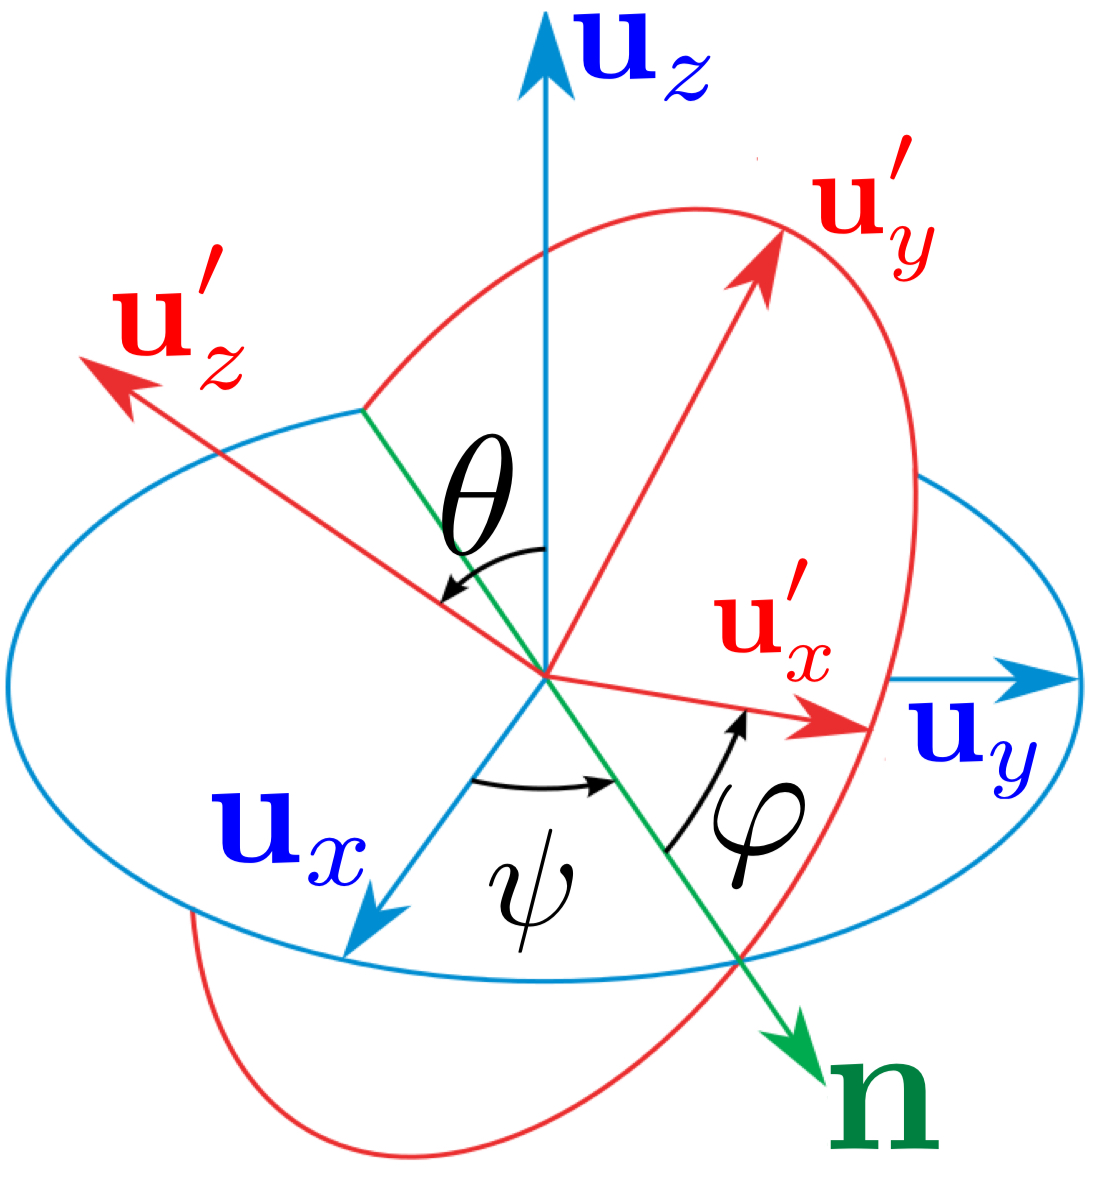
\includegraphics[width=0.07\textwidth]{images/euler.PNG}
  \end{center}
  
  Pour passer de \(\refe\) à \(\refe'\) : 
  \begin{enumerate}
    \item Précéssion : rotation \(\psi\) autour de \(\uz\) pour amener \(\ux\) sur \(\nod\)
    \item Nutation : rotation \(\theta\) autour de \(\nod\), amène \(\uz\) sur \(\uz'\) 
    \item Rotation propre : rotation \(\varphi\) autour de \(\uz'\), amène \(\nod\) sur \(\ux'\) 
  \end{enumerate}

  \subsubsection{Vitesse et acceleration d'un point du solide}
  \[\vi_p=\vi_{O'}+\vian\times\vv{O'P}\]
  \[\ac_p=\ac_{O'}+\diff{\vian}{t}\times\vv{O'P}+\vian\times(\vian\times\vv{O'P})\]

  En utilisant un repère cylindrique on on peut dire que \(\vian\times\vv{O'P}=r\diff{\theta}{t}\utheta\) 

  On remarque aussi que \(\vian = \dot{\psi}\uz + \dot{\theta}\nod + \dot{\varphi}\uz'\)

  \subsubsection{Dynamique d'un corps solide}
  \begin{itemize}
    \item Thm du centre de masse : \( M\ac_G = \F^{\exte} \)
    \item Thm du moment cinétique : 
      \begin{enumerate}
        \item \(\diff{\mc_O}{t} = \mf_O^{\exte}\) (\(O\) doit être fixe)
        \item \(\diff{\mc_G}{t} = \mf_G^{\exte}\)
      \end{enumerate} 
    \item Equation de l'énergie : \(\Delta K = W^{\exte}\)
  \end{itemize}

  \subsection{Rotation autour d'un axe de symétrie \(\Delta_G\)}
  \[
    \exists \Delta_G \Leftrightarrow \forall P_i, \exists P_i' \text{ tq. } 
    \begin{cases}
      \vv{GP}_{i\parallel}=\vv{GP}_{i\parallel}'\\
      \vv{GP}_{i\bot}=-\vv{GP}_{i\bot}'\\
    \end{cases}
  \]

  \subsubsection{Moment cinétique}
  Valable seulement autour d'un axe de symétrie : 
  \[
    \diff{\mc_G}{t} = \diff{}{t}(I_{\Delta G}\vian)=\mf^{\exte}_G
  \]
  \subsubsection{Energie cinétique}
  \[
    K = K_c + K_r = \tfrac{1}{2}Mv_G^2 + \tfrac{1}{2}I_{\Delta_G}\omega^2
  \]

  \subsection{Rotation autour d'un axe instantané fixe (=sans vitesse) \(\Delta \parallel \Delta_G\)}
  \(O\) est la projection de \(G\) sur \(\Delta\).

  Théorème de Huygens-Steiner : 
  \[
    I_{\Delta} = Md^2 + I_{\Delta_G}
  \]
  \[
    \diff{\mc_O}{t} = \diff{}{t}(I_{\Delta}\vian) = I_{\Delta}\diff{\vian}{t}=\mf_O^{\exte}
  \]

  \textbf{Roulement sans glissement : } vitesse instantané du point de contact est égale à 0, malgré le fait que le point de contact change (+ force de frottement statique).

  \section{Solide quelconque}
  \req{1}{
    \delta_{\alpha\beta}=
    \begin{cases}
      0\phantom{tex}\text{si} \phantom{tex}\alpha\neq\beta\\
      1\phantom{tex}\text{si} \phantom{tex}\alpha=\beta\\
    \end{cases}
  }
  \[
    \diff{\mc_G}{t}=\diff{}{t}(\widetilde{I}_G\vian)=\mf_G^{\exte}
  \]
  \[
    \ti_{G,\alpha\beta}=\sum_im_i\left[||\vv{GP}_i||^2\delta_{\alpha\beta} - GP_{i,\alpha}GP_{i,\beta}\right]
  \]
  \[
    K_r = \tfrac{1}{2}M||\vi_G||^2 + \tfrac{1}{2}\omega^{\bot}\ti_G\omega
  \]
  \[
    \omega^{\bot}\ti_G\omega=\mc_G\cdot\vian
  \]

  Si les axes sont parallèles a des axes de symétrie alors on a plus que des composantes sur la diagonale. Pour retrouver dans les coordonées que l'on veut on prend nos axes tel que \(\ti_G'\) soit diagonale et on compute \(\mc_G'=\ti_G'\cdot\vian'\). Puis on reprojette chaque axe sur ceux que l'on veut : \(\mc_G=\left(\mc_G'\cdot\ux\right)\ux + \left(\mc_G'\cdot\uy\right)\uy + \left(\mc_G'\cdot\uz\right)\uz\)

  \subsection{Si \(O\) ne bouge pas}
  \[
    \diff{\mc_O}{t}=\diff{}{t}(\widetilde{I}_O\vian)=\mf_O^{\exte}
  \]
  \[
    \ti_{O,\alpha\beta}=M\left[||\vv{OP}_i||^2\delta_{\alpha\beta} - GP_{i,\alpha}GP_{i,\beta}\right] + \ti_{G,\alpha\beta}
  \]
  \[
    K =\tfrac{1}{2}\omega^{\bot}\ti_O\omega
  \]
  \subsection{Les formules utiles}
  \[
    M\ac = \sum\F^{\exte} \phantom{text} \Delta K = W^{\exte}
  \]
  \[
    \diff{\mc_G}{t}=\mf_G^{\exte} \phantom{text} \diff{\mc_O}{t}=\mf_O^{\exte}
  \]

  \[ \forall P\in \text{ solide } 
    \begin{cases}
      \mc_O = \vv{OG}\times m\vi_G + \mc_G \\
      \vi_P = \vi_G + \Vian\times\vv{GP}
    \end{cases}
  \]

  \[
    \ac_G = \diff[2]{\vv{OG}}{t}
  \]
  \[
    K = \tfrac{1}{2}M\vi_A^2 + M\vi_A\left(\vian\times\vv{AG}\right) + \tfrac{1}{2}\vian\left(\ti_G\vian\right)
  \]

  Position centre de masse : \(\displaystyle \vv{OG}=\frac{\sum_im_i\pos_i}{\sum_im_i}\)

  où \(\displaystyle x_G = \frac{1}{M}\int x\dee m\) 

  % Masses constantes : 

  \(\displaystyle \vi_G = \diff{\pos_G}{t}=\frac{\qm}{M}\phantom{text}\F_{\exte}=\diff{\qm}{t}=M\ac_G\)

  \[\text{EdM d'un solide :}
    \begin{cases}
      \text{3 eq CDM : }m\dot{\vi}_G=\sum\F_{\exte}\\
      \text{3 eq TMC : }\diff{\mc_G}{t}=\mf_G
    \end{cases}
  \]

  Energie mécanique d'un solide : Toutes les forces qui sont au point de contact ne sont pas prisent en compte dans \(E_m\) (travaillent pas parce que la vitesse au point d'application est nulle).

  \subsection{Les cas particulier}
  Pour une force d'inertie d'un solide entier il faut d'abord le faire pour une masse quelconque \(m\) sur le solide puis le généraliser. Exemple d'une tige : Soit \(\displaystyle\mu=\frac{M}{L}\) avec \(M\) la masse d'un solide et \(L\) sa longueur. ON calcule la force d'inertie à une distance \(\rho\) du point pour une masse \(m\) quelconque : \(\dee \F_{ie}=\alpha(\theta,\rho)m\) avec \(\alpha(\theta, \rho)\) une fonction quelconque. Puis on remplace \(m=\mu\dee \rho\) puis on intègre : 
  \[
    \F_{ie} = \int_0^L \dee\F_{ie} = \int_0^L\alpha(\theta,\rho)\mu\dee\rho
  \]

  \section{Kepler}
  \[
    \diff{\mathcal{A}}{t}=\frac{||\vv{L}_0||}{2m}=\text{const} \phantom{text} \frac{a_A^3}{T_A^2}=\frac{a_B^3}{T_B^2}\phantom{text} \frac{T^2}{R^2}=\frac{4 \pi^2}{G(M_s + M)}
  \]
  \(a_A\approx R_A\) pour un cercle
  \section{Chocs}
  \[
    \Qm^{in}=\Qm^{fin} \phantom{texttext}
    \mc^{in}_O=\mc^{fin}_O
  \]
  \[ \Delta K \overset{?}{=}
    \begin{cases}
      0 = \implies \text{choc élastique}\\
      0 \neq \implies \text{choc inélastique}
    \end{cases}
  \]

  Il y a \textbf{choc mou} lorsque les deux masses se collent. La conservation de la quantité de mouvement est vérifié mais \(\Delta K \neq 0\).

  \subsection{Choc 1-D, élastique}
  \[
    \begin{cases}
      m_1 v_{1i} + m_2v_{2i} = m_1 v_{1f} + m_2 v_{2f} \\ 
      \tfrac{1}{2}m_1 v_{1i}^2 + \tfrac{1}{2}m_1 v_{2f}^2 - \tfrac{1}{2}m_1 v_{1f}^2 = 0
    \end{cases}
  \]

  Ce système a pour solutions :
  \[
    \begin{cases}
      v_{1f} = \frac{(m_1-m_2)v_{1i} + 2m_2v_{2i}}{m_1+m_2} \\
      v_{2f} = \frac{(m_2-m_1)v_{2i} + 2m_1v_{1i}}{m_1+m_2}
    \end{cases}
  \]

  \subsection{Choc inélastique}
  \[
    \Delta K 
    \begin{cases}
      > 0 \implies \text{exo-énergetique} \\
      < 0 \implies \text{endo-énergetique}
    \end{cases}
  \]

  \subsection{Choc mou (parfaitement inélastique)}
  Les deux objet se collent (\(\vi_{1f}=\vi_{2f}=\vi_{\text{mou}}\)). Dans le cas particulier ou \(\vi_{2i}=0\), la conservation de la quantité de mouvement nous dit que : 
  \[
    m_1\vi_{1i} = m_1\vi_{1f} + m_2\vi_{2f} = (m_1 + m_2)\vi_{\text{mou}} 
  \]
  \[
    \vi_{\text{mou}} = \frac{m_1}{m_1 + m_2}\vi_{1i}
  \]
  \[
    \Delta K = K^{\text{fin}} - K^{\text{in}}= -\tfrac{1}{2}\frac{m_1m_2}{m_1+m_2}v_{\text{mou}}^2 < 0 
  \]

  \section{Système à masses variable}
  \[ M(t)\diff{\vi}{t}=\sum\F^{\text{ext}} + \vi_{\text{rel}}\diff{M}{t} \]

  \section{Moment d'inertie}
  \(\Delta_C=\)axe du cylindre

  \scalebox{0.7}{
    \begin{tabular}{p{3cm}l}
      Boule (pleine) & \(\displaystyle I = \frac{2}{5}mR^2\)\\

      Sphère (creuse) & \(\displaystyle I = \frac{2}{3}mR^2\)\\

      Anneau (\(\Delta_c\)) & \(\displaystyle I = mR^2\)\\

      Anneau (\(\bot\Delta_c\)) & \(\displaystyle I = \frac{1}{2}mR^2\)\\

      Anneau (épaisseur \(\neq 0\), \(\Delta_c\)) & \(\displaystyle I = \frac{1}{2}m(R_1^2 + R_2^2)\)\\

      Cylindre (\(\Delta_c\)) & \(\displaystyle I = \frac{1}{2}mR^2\)\\

      Cylindre (\(\bot\Delta_c\)) & \(\displaystyle I = \frac{1}{4}mR^2 + \frac{1}{12}mL^2\)
    \end{tabular}
  }
\end{multicols}
\end{document}
